\documentclass[11pt,a4paper]{article}
\usepackage[margin=1in]{geometry}
\usepackage{tikz}
\usepackage{amsmath,amssymb}
\usepackage{xcolor}
\usepackage{float}
\usepackage{caption}
\usepackage{subcaption}

% TikZ libraries
\usetikzlibrary{arrows.meta,positioning,calc,backgrounds,patterns,decorations.pathmorphing}

% Define common colors
\definecolor{manifoldcolor}{RGB}{200,50,50}
\definecolor{trajcolor1}{RGB}{50,150,50}
\definecolor{trajcolor2}{RGB}{50,50,200}
\definecolor{perturbcolor}{RGB}{255,140,0}
\definecolor{stablecolor}{RGB}{200,50,50}
\definecolor{unstablecolor}{RGB}{50,200,50}
\definecolor{saddlecolor}{RGB}{200,200,50}
\definecolor{noisycolor}{RGB}{255,140,0}
\definecolor{dropoutcolor}{RGB}{150,50,200}
\definecolor{losscolor}{RGB}{100,150,200}

% Title and author
\title{Loss of Plasticity (LoP) Manifolds:\\TikZ Visualizations}
\author{Mathematical Illustrations of Gradient Descent Traps}
\date{\today}

\begin{document}

\maketitle

\section{Introduction}
This document contains TikZ visualizations illustrating the concept of Loss of Plasticity (LoP) manifolds in neural networks. These manifolds represent regions in parameter space where gradient-based optimization becomes trapped, preventing further learning.

\section{Visualizations}

\subsection{Parameter Space with LoP Manifolds}

\begin{figure}[H]
\centering
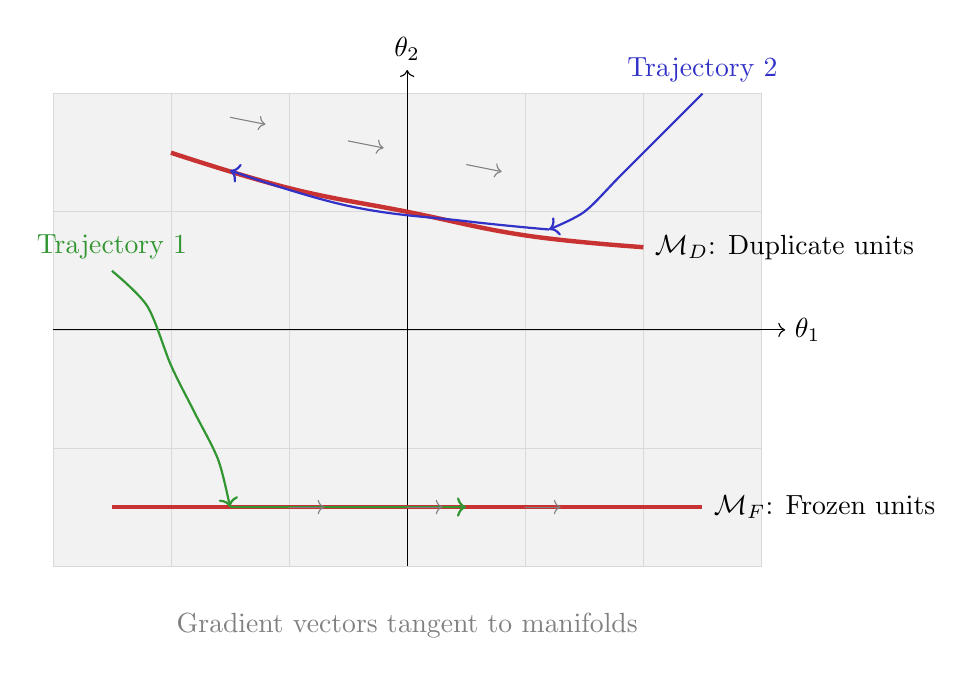
\begin{tikzpicture}[scale=1.5]
    % Draw parameter space background
    \fill[gray!10] (-3,-2) rectangle (3,2);
    
    % Draw grid
    \draw[gray!30,very thin] (-3,-2) grid (3,2);
    
    % Draw axes
    \draw[->] (-3,0) -- (3.2,0) node[right] {$\theta_1$};
    \draw[->] (0,-2) -- (0,2.2) node[above] {$\theta_2$};
    
    % Draw LoP manifold (frozen units manifold)
    \draw[manifoldcolor,ultra thick] (-2.5,-1.5) -- (2.5,-1.5) 
        node[right,black] {$\mathcal{M}_F$: Frozen units};
    
    % Draw LoP manifold (duplicate units manifold)
    \draw[manifoldcolor,ultra thick] plot[smooth,tension=0.7] 
        coordinates {(-2,1.5) (-1,1.2) (0,1) (1,0.8) (2,0.7)}
        node[right,black] {$\mathcal{M}_D$: Duplicate units};
    
    % Draw gradient flow trajectories
    % Trajectory 1: Gets trapped on frozen manifold
    \draw[trajcolor1,thick,->] plot[smooth,tension=0.5] 
        coordinates {(-2.5,0.5) (-2.2,0.2) (-2,-0.3) (-1.8,-0.7) (-1.6,-1.1) (-1.5,-1.5)};
    \draw[trajcolor1,thick,->] (-1.5,-1.5) -- (0.5,-1.5);
    \node[trajcolor1] at (-2.5,0.7) {Trajectory 1};
    
    % Trajectory 2: Gets trapped on duplicate manifold
    \draw[trajcolor2,thick,->] plot[smooth,tension=0.5] 
        coordinates {(2.5,2) (2.2,1.7) (1.8,1.3) (1.5,1) (1.2,0.85)};
    \draw[trajcolor2,thick,->] plot[smooth,tension=0.7] 
        coordinates {(1.2,0.85) (0.5,0.92) (-0.5,1.05) (-1.5,1.35)};
    \node[trajcolor2] at (2.5,2.2) {Trajectory 2};
    
    % Show gradient vectors tangent to manifolds
    \foreach \x in {-1,0,1} {
        \draw[->,gray] (\x,-1.5) -- (\x+0.3,-1.5);
    }
    \foreach \x in {-1.5,-0.5,0.5} {
        \pgfmathsetmacro\y{1.5 - 0.2*\x}
        \pgfmathsetmacro\dy{-0.2}
        \draw[->,gray] (\x,\y) -- (\x+0.3,\y+0.3*\dy);
    }
    
    % Legend
    \node[gray] at (0,-2.5) {Gradient vectors tangent to manifolds};
\end{tikzpicture}
\caption{Gradient descent trajectories getting trapped on LoP manifolds. The frozen units manifold $\mathcal{M}_F$ represents parameters that stop updating due to saturated activations. The duplicate units manifold $\mathcal{M}_D$ represents parameters constrained to maintain unit cloning.}
\end{figure}

\subsection{Stability Types of LoP Manifolds}

\begin{figure}[H]
\centering
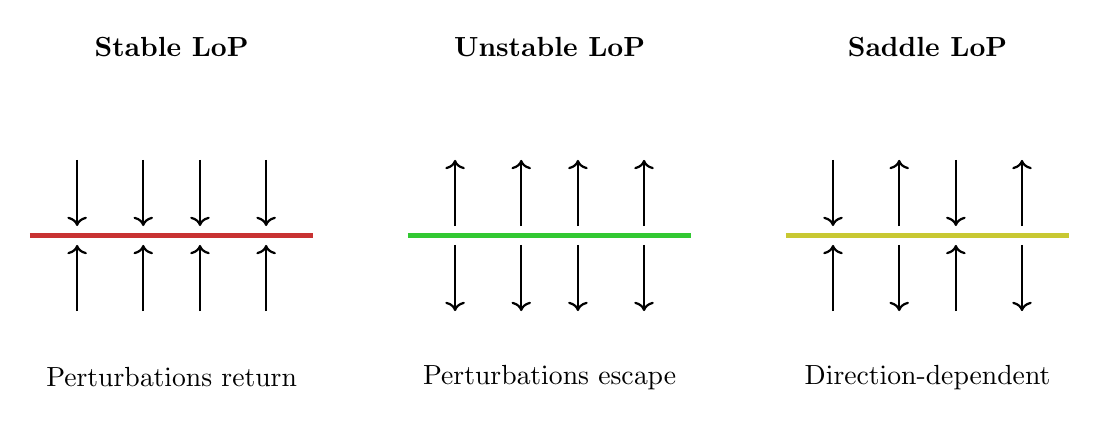
\begin{tikzpicture}[scale=1.2]
    % Stable Manifold
    \begin{scope}[shift={(-4,0)}]
        \node at (0,2) {\textbf{Stable LoP}};
        \draw[stablecolor,ultra thick] (-1.5,0) -- (1.5,0);
        % Perturbation arrows pointing back
        \foreach \x in {-1,-0.3,0.3,1} {
            \draw[->,thick] (\x,0.8) -- (\x,0.1);
            \draw[->,thick] (\x,-0.8) -- (\x,-0.1);
        }
        \node at (0,-1.5) {Perturbations return};
    \end{scope}
    
    % Unstable Manifold
    \begin{scope}[shift={(0,0)}]
        \node at (0,2) {\textbf{Unstable LoP}};
        \draw[unstablecolor,ultra thick] (-1.5,0) -- (1.5,0);
        % Perturbation arrows pointing away
        \foreach \x in {-1,-0.3,0.3,1} {
            \draw[->,thick] (\x,0.1) -- (\x,0.8);
            \draw[->,thick] (\x,-0.1) -- (\x,-0.8);
        }
        \node at (0,-1.5) {Perturbations escape};
    \end{scope}
    
    % Saddle Manifold
    \begin{scope}[shift={(4,0)}]
        \node at (0,2) {\textbf{Saddle LoP}};
        \draw[saddlecolor,ultra thick] (-1.5,0) -- (1.5,0);
        % Mixed perturbation arrows
        \foreach \x in {-1,0.3} {
            \draw[->,thick] (\x,0.8) -- (\x,0.1);
            \draw[->,thick] (\x,-0.8) -- (\x,-0.1);
        }
        \foreach \x in {-0.3,1} {
            \draw[->,thick] (\x,0.1) -- (\x,0.8);
            \draw[->,thick] (\x,-0.1) -- (\x,-0.8);
        }
        \node at (0,-1.5) {Direction-dependent};
    \end{scope}
\end{tikzpicture}
\caption{Three types of LoP manifold stability. Stable manifolds actively trap gradient descent, unstable manifolds allow easy escape, and saddle manifolds show mixed behavior depending on perturbation direction.}
\end{figure}

\subsection{Escape Mechanisms from LoP Manifolds}

\begin{figure}[H]
\centering
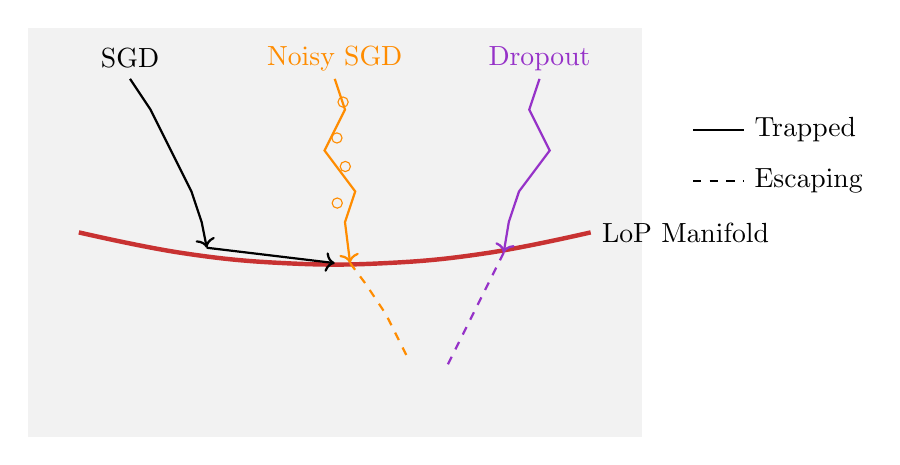
\begin{tikzpicture}[scale=1.3]
    % Background
    \fill[gray!10] (-3,-2) rectangle (3,2);
    
    % Draw manifold
    \draw[manifoldcolor,ultra thick] plot[smooth,tension=0.7] 
        coordinates {(-2.5,0) (-1.5,-0.2) (-0.5,-0.3) (0.5,-0.3) (1.5,-0.2) (2.5,0)}
        node[right,black] {LoP Manifold};
    
    % Standard gradient descent (trapped)
    \draw[black,thick,->] (-2,1.5) -- (-1.8,1.2) -- (-1.6,0.8) -- (-1.4,0.4) -- (-1.3,0.1) -- (-1.25,-0.15);
    \draw[black,thick,->] (-1.25,-0.15) -- (0,-0.3);
    \node[black] at (-2,1.7) {SGD};
    
    % Noisy SGD (escaping)
    \draw[noisycolor,thick,->] (0,1.5) -- (0.1,1.2) -- (-0.1,0.8) -- (0.2,0.4) -- (0.1,0.1) -- (0.15,-0.3);
    \draw[noisycolor,thick,dashed] (0.15,-0.3) -- (0.3,-0.5) -- (0.5,-0.8) -- (0.7,-1.2);
    \node[noisycolor] at (0,1.7) {Noisy SGD};
    
    % Dropout (escaping)
    \draw[dropoutcolor,thick,->] (2,1.5) -- (1.9,1.2) -- (2.1,0.8) -- (1.8,0.4) -- (1.7,0.1) -- (1.65,-0.2);
    \draw[dropoutcolor,thick,dashed] (1.65,-0.2) -- (1.5,-0.5) -- (1.3,-0.9) -- (1.1,-1.3);
    \node[dropoutcolor] at (2,1.7) {Dropout};
    
    % Add noise symbols
    \foreach \i in {1,2,3,4} {
        \pgfmathsetmacro\x{0.1 + 0.1*rand}
        \pgfmathsetmacro\y{1.5 - 0.3*\i + 0.1*rand}
        \draw[noisycolor,thin] (\x,\y) circle (0.05);
    }
    
    % Legend
    \draw[black,thick] (3.5,1) -- (4,1) node[right] {Trapped};
    \draw[dashed,thick] (3.5,0.5) -- (4,0.5) node[right] {Escaping};
\end{tikzpicture}
\caption{Different optimization methods interacting with LoP manifolds. Standard SGD gets trapped, while Noisy SGD and Dropout can escape through perturbations that break the manifold constraints.}
\end{figure}

\subsection{3D Conceptual View of LoP Manifolds in Loss Landscape}

\begin{figure}[H]
\centering
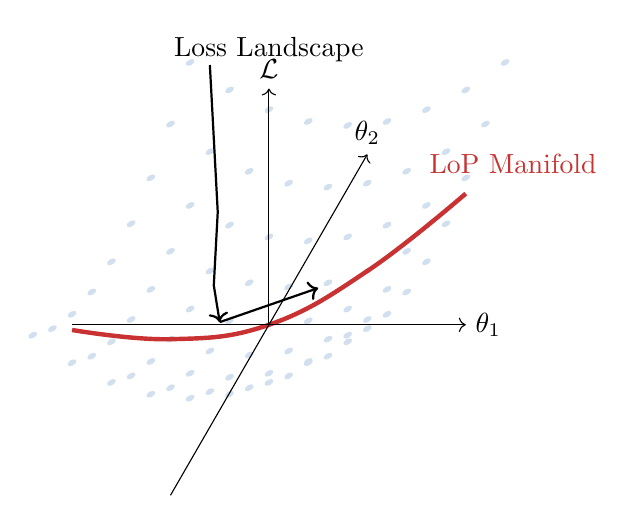
\begin{tikzpicture}[scale=1,
    x={(1cm,0cm)},
    y={(0.5cm,0.866cm)},
    z={(0cm,1cm)}]
    
    % Draw loss surface (simplified)
    \foreach \x in {-2,-1.5,...,2} {
        \foreach \y in {-2,-1.5,...,2} {
            \pgfmathsetmacro\z{0.2*(\x*\x + \y*\y)}
            \fill[losscolor!30] (\x,\y,\z) circle (0.05);
        }
    }
    
    % Draw LoP manifold as a valley
    \draw[manifoldcolor,ultra thick] plot[smooth,tension=0.7]
        coordinates {(-2,-1,0.8) (-1,-0.5,0.25) (0,0,0) (1,0.5,0.25) (2,1,0.8)};
    
    % Draw gradient trajectories
    \draw[black,thick,->] (-1.5,1.5,2) -- (-1.2,1,1.5) -- (-0.9,0.5,1) -- (-0.7,0,0.5) -- (-0.5,-0.25,0.25);
    \draw[black,thick,->] (-0.5,-0.25,0.25) -- (0.5,0.25,0.25);
    
    % Draw coordinate frame
    \draw[->] (-2.5,0,0) -- (2.5,0,0) node[right] {$\theta_1$};
    \draw[->] (0,-2.5,0) -- (0,2.5,0) node[above] {$\theta_2$};
    \draw[->] (0,0,0) -- (0,0,3) node[above] {$\mathcal{L}$};
    
    % Labels
    \node[manifoldcolor] at (2.5,1.2,1) {LoP Manifold};
    \node at (0,0,3.5) {Loss Landscape};
\end{tikzpicture}
\caption{3D visualization showing how LoP manifolds appear as valleys in the loss landscape where gradient flow becomes confined.}
\end{figure}

\subsection{Network Architecture View of Frozen and Duplicate Units}

\begin{figure}[H]
\centering
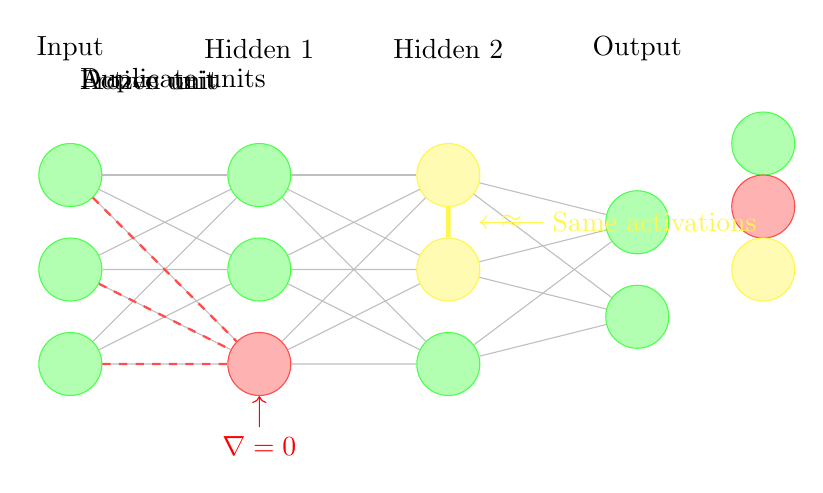
\begin{tikzpicture}[scale=0.8]
    % Define styles
    \tikzstyle{neuron}=[circle,draw,minimum size=0.8cm]
    \tikzstyle{frozen}=[neuron,fill=red!30,draw=red!70]
    \tikzstyle{active}=[neuron,fill=green!30,draw=green!70]
    \tikzstyle{duplicate}=[neuron,fill=yellow!30,draw=yellow!70]
    
    % Input layer
    \foreach \i in {1,2,3} {
        \node[active] (in\i) at (0,-\i*1.5) {};
    }
    \node at (0,0.5) {Input};
    
    % Hidden layer 1
    \foreach \i in {1,2} {
        \node[active] (h1\i) at (3,-\i*1.5) {};
    }
    \node[frozen] (h13) at (3,-4.5) {};
    \node at (3,0.5) {Hidden 1};
    
    % Hidden layer 2
    \node[duplicate] (h21) at (6,-1.5) {};
    \node[duplicate] (h22) at (6,-3) {};
    \node[active] (h23) at (6,-4.5) {};
    \node at (6,0.5) {Hidden 2};
    
    % Output layer
    \node[active] (out1) at (9,-2.25) {};
    \node[active] (out2) at (9,-3.75) {};
    \node at (9,0.5) {Output};
    
    % Draw connections
    \foreach \i in {1,2,3} {
        \foreach \j in {1,2,3} {
            \draw[gray!50] (in\i) -- (h1\j);
        }
    }
    \foreach \i in {1,2,3} {
        \foreach \j in {1,2,3} {
            \draw[gray!50] (h1\i) -- (h2\j);
        }
    }
    \foreach \i in {1,2,3} {
        \foreach \j in {1,2} {
            \draw[gray!50] (h2\i) -- (out\j);
        }
    }
    
    % Highlight frozen connections
    \foreach \i in {1,2,3} {
        \draw[red!70,thick,dashed] (in\i) -- (h13);
    }
    
    % Highlight duplicate connections
    \draw[yellow!70,ultra thick] (h21) -- (h22);
    \node[yellow!70] at (7,-2.25) {$\approx$};
    
    % Legend
    \node[active] at (11,-1) {} node[right] {Active unit};
    \node[frozen] at (11,-2) {} node[right] {Frozen unit};
    \node[duplicate] at (11,-3) {} node[right] {Duplicate units};
    
    % Annotations
    \draw[<-,red] (h13) -- ++(0,-1) node[below] {$\nabla = 0$};
    \draw[<-,yellow!70] (6.5,-2.25) -- ++(1,0) node[right] {Same activations};
\end{tikzpicture}
\caption{Network architecture showing how LoP manifests at the unit level. Frozen units have zero gradients due to saturated activations, while duplicate units produce identical outputs, reducing the network's effective capacity.}
\end{figure}

\section{Mathematical Background}

\subsection{LoP Manifold Definition}
A manifold $\mathcal{M} \subset \Theta$ induces Loss of Plasticity if the gradient of the loss function is tangent to the manifold at every point:
$$\nabla_\theta \mathcal{L}(\theta) \in T_\theta\mathcal{M} \quad \forall \theta \in \mathcal{M}$$
where $T_\theta\mathcal{M}$ denotes the tangent space of $\mathcal{M}$ at $\theta$.

\subsection{Types of LoP Manifolds}
\begin{itemize}
    \item \textbf{Frozen Units Manifold ($\mathcal{M}_F$)}: Parameters corresponding to saturated units where activation derivatives are zero.
    \item \textbf{Duplicate Units Manifold ($\mathcal{M}_D$)}: Parameters constrained to maintain identical computations across multiple units.
\end{itemize}

\subsection{Stability Classifications}
\begin{itemize}
    \item \textbf{Stable LoP}: $v^\top\nabla_\theta^2\mathcal{L}(\theta)v > 0$ for all $v \in N_\theta\mathcal{M}\setminus\{0\}$
    \item \textbf{Unstable LoP}: $v^\top\nabla_\theta^2\mathcal{L}(\theta)v < 0$ for all $v \in N_\theta\mathcal{M}\setminus\{0\}$
    \item \textbf{Saddle LoP}: Mixed positive and negative curvature in normal directions
\end{itemize}

\section{Compilation Instructions}
To compile this document:
\begin{verbatim}
pdflatex lop_manifold_visualizations.tex
\end{verbatim}

Required packages: \texttt{tikz}, \texttt{amsmath}, \texttt{amssymb}, \texttt{xcolor}, \texttt{float}, \texttt{caption}, \texttt{subcaption}.

\end{document}